\section{System Design}
\label{sec:design}

% 中文导读（仅供写作与审阅，不进入最终 PDF）：
% 本节围绕“workflow 紧迫度 -> chunk 放置 -> HBM 配额调节 -> 故障恢复”这一闭环展开。
% 首先给出 DP=2、PP=2 的总体架构和保护对象，明确逻辑 Master 只管理路由、放置和恢复元数据，
% KV tensor 由同 stage worker 与共享 DRAM/SSD 数据路径直接传输。随后分别介绍：


% Algorithm 1 如何根据已揭示 workflow DAG 传播 Slack
% Algorithm 2
% Landlord Online Caching Algorithm
% Minimum-Cost Flow（MCF，最小费用流）
% Algorithm 3
% TCP-style Additive Increase/Multiplicative Decrease（AIMD，加性增大/乘性减小）

% 本节共有两组图像：

% 1. Figure~\ref{fig:architecture}（figures/system-design.pdf）：
%    展示 Application、Router/AegisKV Control Plane、Inference Engine/Shared KV Tiers 三层架构，
%    包括 DP=2、PP=2 进程拓扑、Algorithm 1/2/3 的实现位置、同 stage Peer HBM 路径以及共享 DRAM/SSD。
% 2. Figure~\ref{fig:commit-recovery}（figures/commit-recovery-protocol.pdf）：
%    展示 chunk 的分 stage 放置、保护状态形成和 GPU 故障后的整请求恢复过程，用于解释控制元数据与 KV 数据路径的关系。

\subsection{Overview}

The design follows three coupled decisions.  Algorithm~1 estimates each
request's workflow slack, Algorithm~2 chooses a protection tier for completed
KV chunks, and Algorithm~3 adjusts the HBM budget that Algorithm~2 may use.
\system{} separates these policies from transfer.  An application-side workflow
handler reports DAG progress and causal slack (Algorithm~1).  The router freezes
an execution DP $e(r)$, one complete backup DP $b(r)$ in a distinct GPU failure
domain, and a route version for each request.  A logical master maintains
versioned KV metadata, solves a
chunk-placement problem at each completed-chunk event (Algorithm~2), and
publishes a slower-timescale, versioned per-DP peer-HBM admission envelope
$\alpha$ (Algorithm~3).
Scheduler/worker processes execute the plan and
transfer bytes through peer-to-peer GPU paths, a shared DRAM pool, or SSD.  The
master is not on the data path.

\begin{figure*}[t]
  \centering
  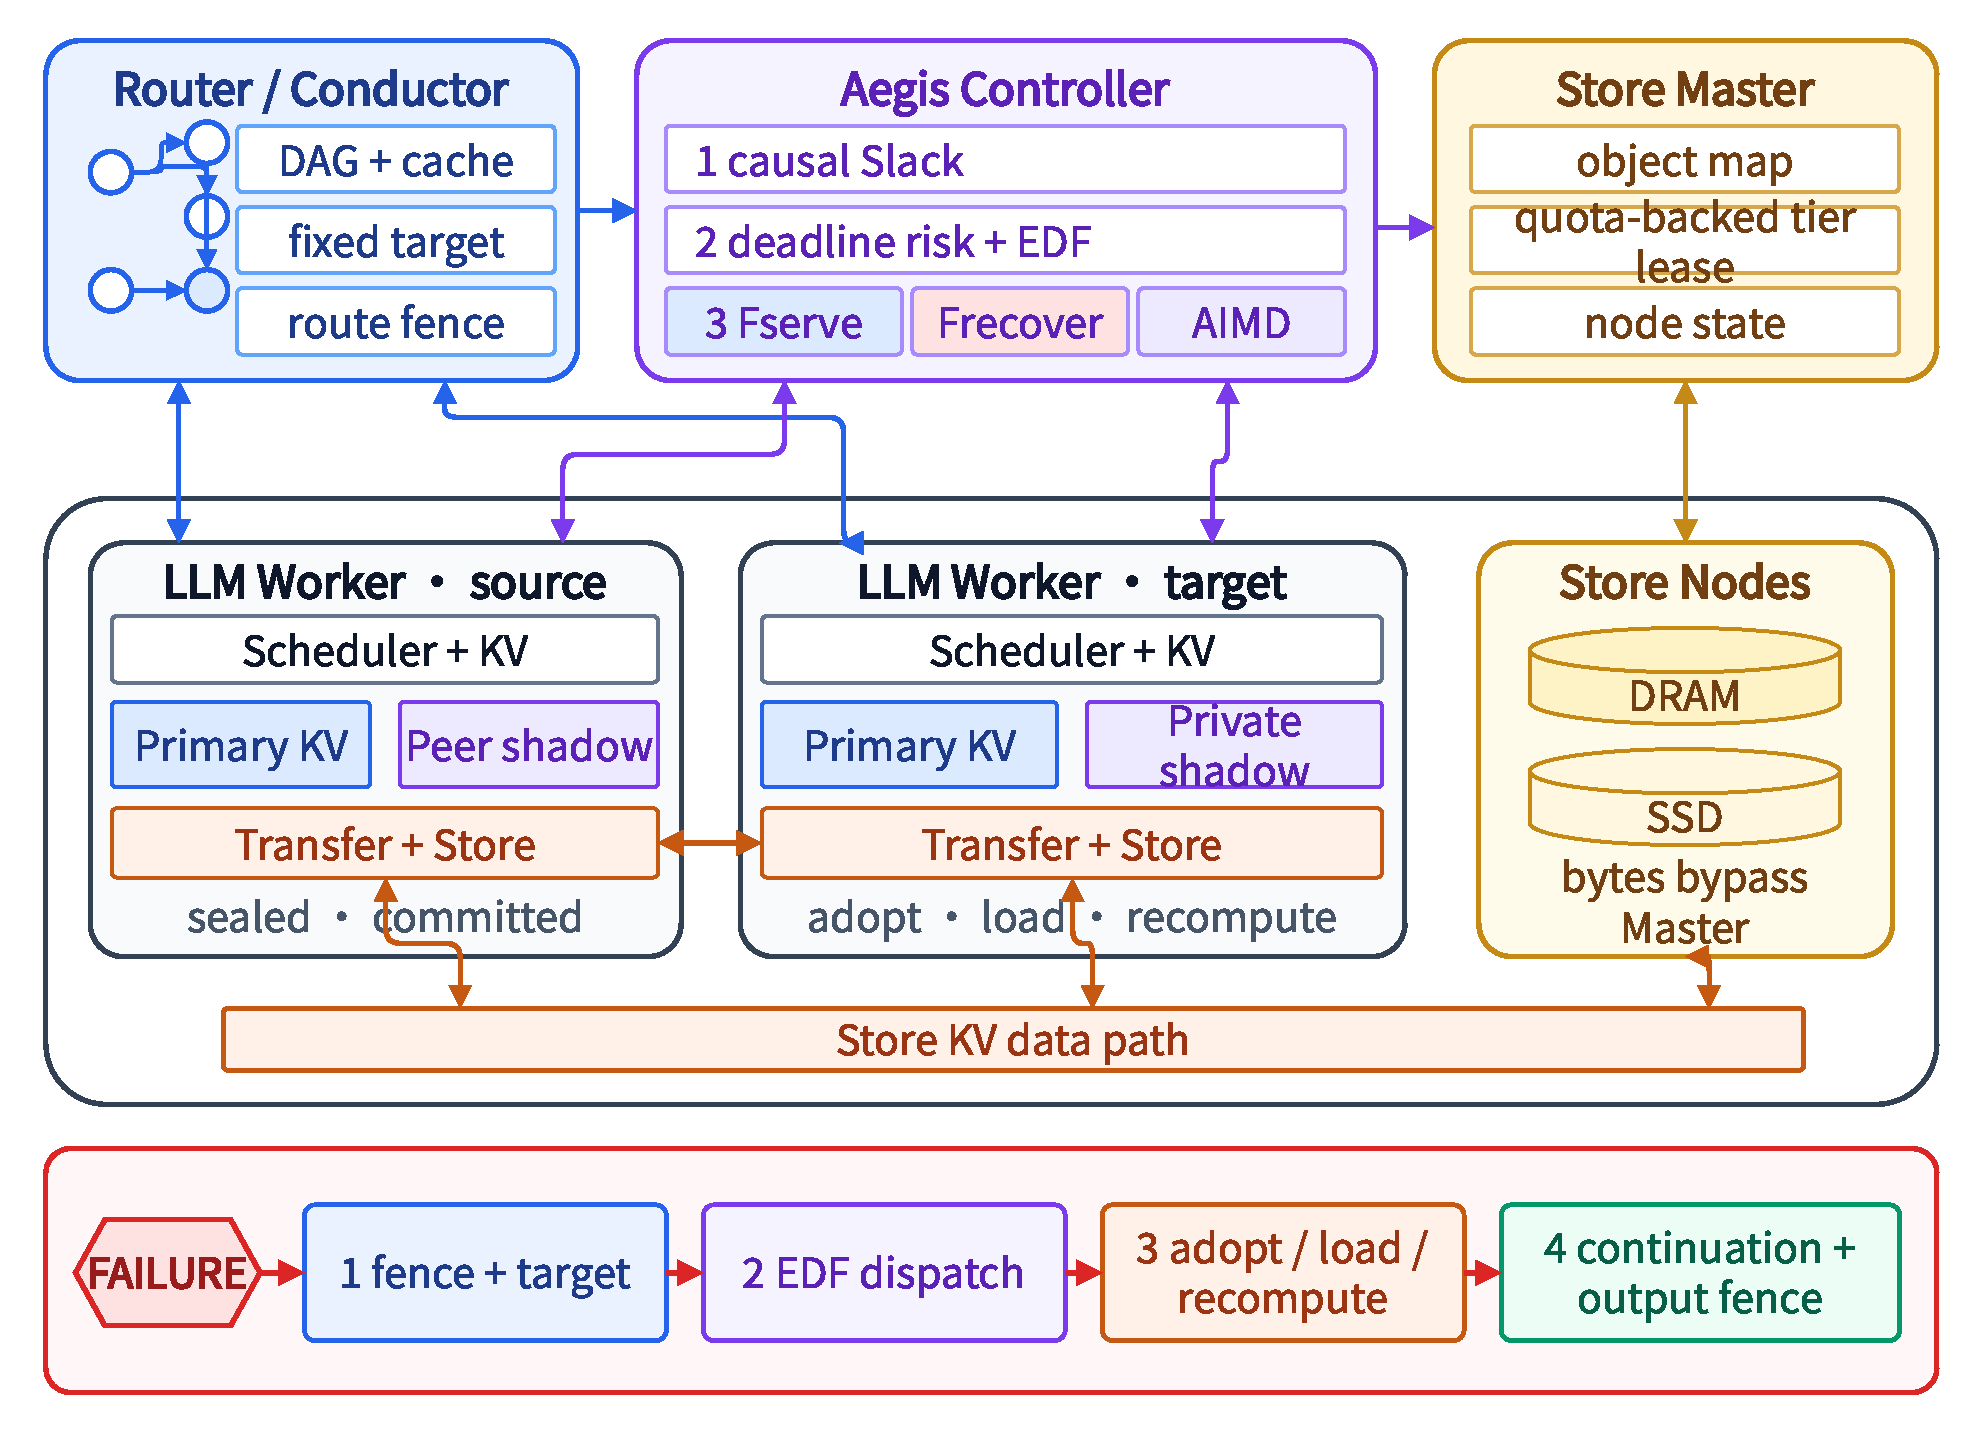
\includegraphics[width=0.96\textwidth]{figures/system-design.pdf}
  \caption{\system{} architecture.  A logical master owns placement, commit,
  and per-DP HBM admission, while matching-stage workers and shared DRAM/SSD
  stores move KV bytes.  The illustrated $D=2$, $P=2$ deployment uses one
  versioned $\alpha$ envelope per DP and preserves PP-stage identity on every
  KV path; the master never relays KV tensors.}
  \Description{A control plane sends per-request slack, per-chunk placement,
  and per-DP HBM admission envelopes to data-parallel pipeline workers; the data plane
  transfers stage-aligned KV chunks to peer HBM, DRAM, or SSD.}
  \label{fig:architecture}
\end{figure*}

The target serving topology contains $D$ DP replicas and $P$ pipeline-parallel
(PP) stages per replica.  A request enters PP stage~0 of one DP, and all stages
advance that request through an ordered pipeline.  Figure~\ref{fig:architecture}
uses $D=2$, $P=2$, and tensor parallelism one, yielding four independently
supervised scheduler/worker processes; larger deployments repeat the same
mapping.  Each process owns only its layer interval and corresponding KV
bytes.  Consequently, a chunk created at source $(e(r),p)$ can be copied to
stage $p$ of the request's frozen $b(r)$ or to a tier that preserves stage
identity; copying it to stage $p'\ne p$ is invalid.

The router is outside Algorithm~2, but its output obeys a concrete contract.
It chooses $e(r)$ and $b(r)$ from healthy, model- and layout-compatible complete
replicas in distinct failure domains, using registered load and failover
headroom estimates.  For every enumerated scenario, the destination must pass
both per-stage HBM admission and retry-service-capacity guards.  If no such
destination exists, the request is not eligible for peer-HBM protection and
the system records that the route contract is degraded.  All optimization
claims below are conditional on these frozen routes and their registered
capacity estimates; Algorithm~2 does not retroactively choose a more favorable
backup DP.

\subsection{Protection object and invariants}
\label{sec:object}

The unit of policy is a \emph{logical KV chunk}.  Its immutable content key is
\begin{equation}
  i=\langle w,r,u,c,e_c,h_{\mathrm{layout}}\rangle,
  \label{eq:chunk-id}
\end{equation}
where $w$ is workflow, $r$ request, $u$ turn, $c$ monotonically increasing
chunk index, $e_c$ an immutable content epoch, and $h_{\mathrm{layout}}$ a hash
of the model, KV layout, and token interval.  A separate route/manifest epoch
$v_r$ binds this content to $e(r)$, $b(r)$, and its placement vector.  Separating
content from routing lets a successor manifest reference a surviving DRAM/SSD
object by its content key without pretending that the object was rewritten
under the new route epoch.
Each PP stage stores a shard $i_p$ containing the KV tensors for its layers and
the chunk's token interval.  Metadata records each shard's size, checksum,
tier, destination, creation time, and acknowledgement state.  The token
sequence, sampling state, and client-visible output commit offset needed to
continue decode are logged with the request version in failure-isolated host or
shared-store memory.  Before a generated token becomes externally visible, its
token ID and output offset enter this compact log.  This logging traffic is
charged to the protection cost and isolation guard; KV bytes alone are
insufficient to reproduce a request or avoid duplicate streamed output.

For tier $\ell$ and stage $p$, let $A_{i,p}^{\ell}=1$ only after the
destination validates the chunk identity, version, and token interval.  A
logical chunk is committed iff every required stage has at least one surviving
acknowledged shard:
\begin{equation}
  A_i=\bigwedge_{p=0}^{P-1}
      \left(\bigvee_{\ell\in\{H,D,S\}} A_{i,p}^{\ell}\right).
  \label{eq:all-stage-ack}
\end{equation}
The stage shards may occupy different tiers; for example, stages 0 and 1 may
reside in DRAM while stages 2 and 3 use peer HBM.  Let $C_r$ be the largest
completed chunk index for request $r$.  Chunks are indexed from one; index zero
is a sentinel denoting reproducible input with no protected decode chunk.  For
a request and route version, the safe frontier is the largest
contiguous prefix of committed chunks:
\begin{equation}
  \safe_r = \max\left\{f\in\{0,\ldots,C_r\}:\;
    \prod_{c=1}^{f} A_{r,c}=1\right\}.
  \label{eq:safe-frontier}
\end{equation}
Here $A_{r,c}$ abbreviates $A_i$ for the request's active route version, and
the empty product at $f=0$ is one.
Operationally the frontier is the minimum version-matched committed frontier across
all required PP stages.  Aggregate byte counters cannot advance it.  Out-of-
order completions may become usable later, but never create a hole-spanning
recovery point.

The protocol maintains four invariants: (1) route, version, and token boundaries
are immutable within a transfer; (2) each shard preserves its PP-stage identity,
and every peer-HBM copy is outside the source failure domain; (3) only the
master advances $\safe_r$ after validating Equation~\ref{eq:all-stage-ack} and
prefix continuity; and (4) workers reject stale plans after an epoch change.
A transfer interrupted by failure can leave orphan bytes, which are reclaimed
by lease expiry and are never advertised as recoverable.

\begin{figure*}[t]
  \centering
  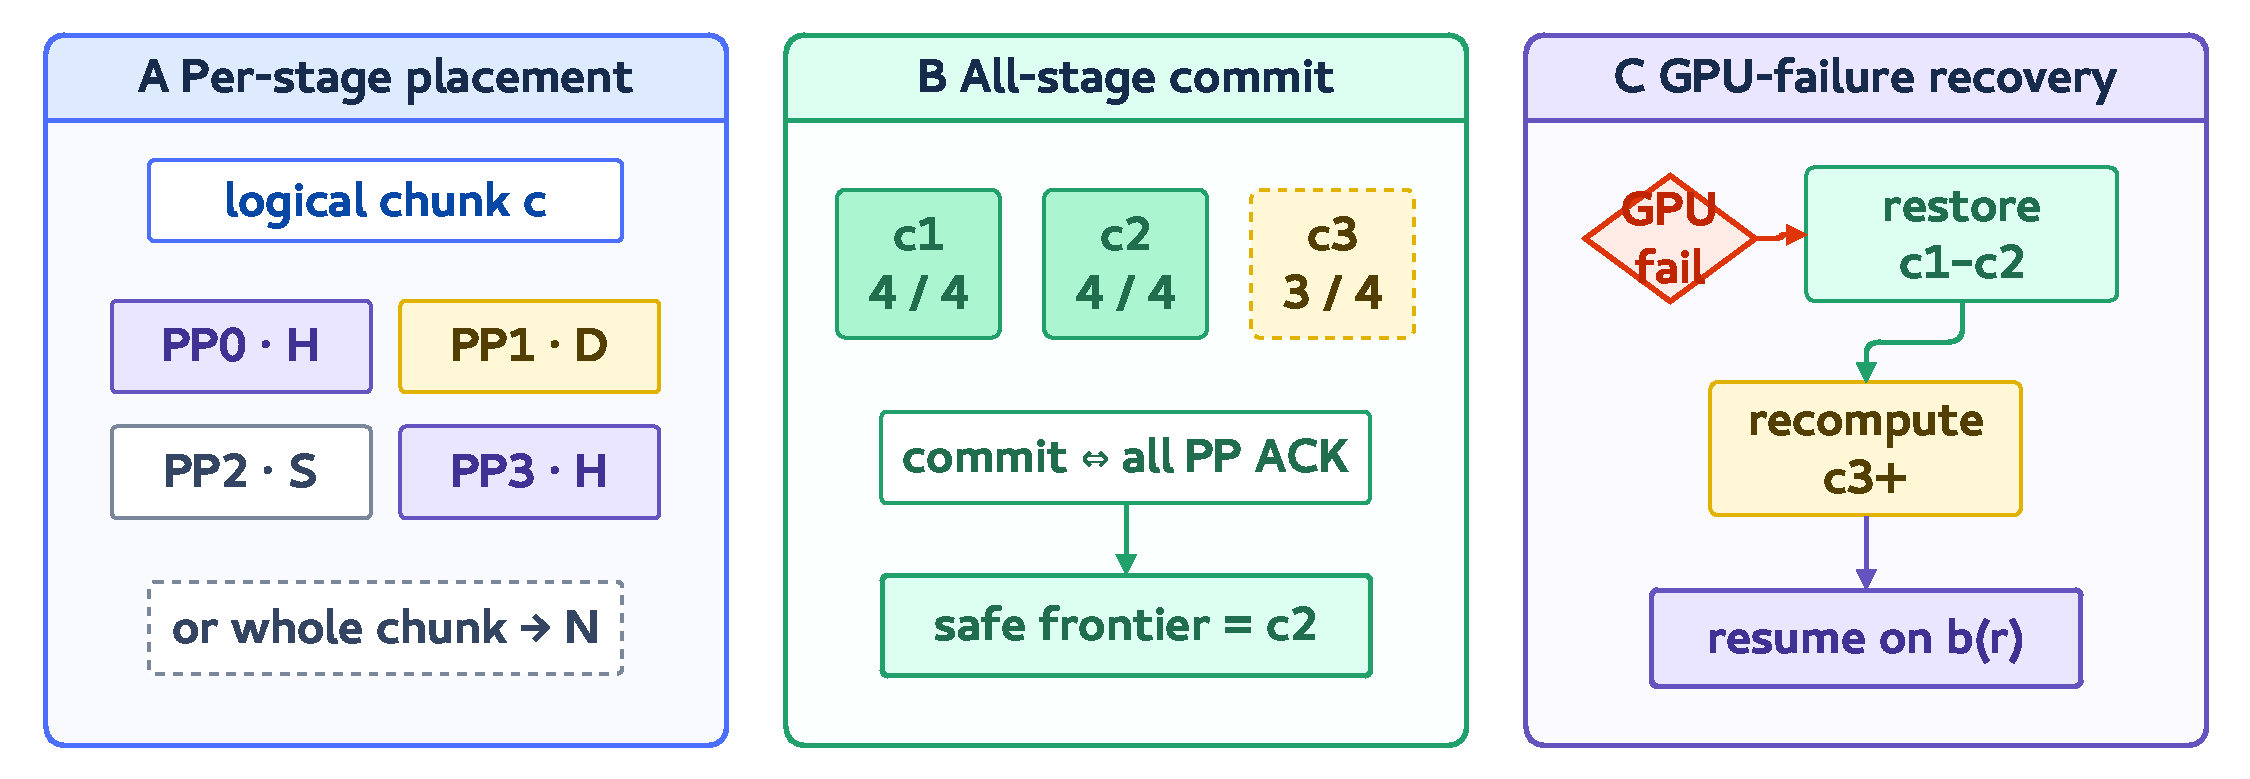
\includegraphics[width=0.96\textwidth]{figures/commit-recovery-protocol.pdf}
  \caption{Protection and recovery contract.  A protected chunk assigns every
  required stage to HBM, DRAM, or SSD; otherwise the whole chunk is
  $N$/Recompute.  All-stage ACKs advance a contiguous safe frontier, which
  bounds restoration before suffix recomputation on the frozen backup DP.}
  \Description{Three panels show mixed per-stage placement, an all-stage ACK
  barrier forming a contiguous safe frontier, and whole-request recovery on a
  frozen backup replica after a GPU failure.}
  \label{fig:commit-recovery}
\end{figure*}

\subsection{Algorithm 1: causal slack propagation}
\label{sec:alg1}

The workflow handler updates Equation~\ref{eq:slack} at request admission, DAG
events, and periodic control epochs.  Before routing it emits
$\langle w,r,k_s,s_r\rangle$, where $k_s$ is a monotonically increasing
slack-sample epoch.  The serving router then freezes $e(r)$, $b(r)$, and route
epoch $v_r$, and creates the request contract
$\langle w,r,v_r,k_s,s_r\rangle$.  The route remains immutable within $v_r$,
but Algorithm~1 may publish a newer $k_s$ as the revealed DAG changes; the
master binds it to the existing route contract and Algorithm~2 ignores stale
slack samples.  Later PP stages learn the route epoch through the ordered
pipeline channel and do not independently admit or reroute a copy.

The remaining-path estimator can be instantiated by a quantile model over node
type, prompt length, observed output tokens, tool class, and queue state.  Its
interface is intentionally narrow: Algorithm~2 consumes a versioned revealed-DAG
timing summary, slack, and an uncertainty bound, not application-specific
``importance'' labels.  To avoid a policy that
is overconfident under distribution shift, a conservative deployment subtracts
an error margin $q_r$:
\begin{equation}
  s_r^{-}(t)=\left[s_r(t)-q_r(t)\right]_+.
  \label{eq:robust-slack}
\end{equation}
When uncertainty is unavailable, the system uses measured calibration error
from a preceding window.  This mechanism changes urgency but cannot override
the hard isolation constraints below.

\subsection{Algorithm 2: three physical tiers or logical Recompute}
\label{sec:alg2}

Within slow-control window $k$, every chunk completion becomes eligible for an
Algorithm~2 decision; resource and failure events can invalidate a plan.  To
avoid one global solve per completion, the master coalesces events for at most
a registered $T_{\mathrm{wait}}$, solves asynchronously from the last incumbent
with warm-started state over a causal horizon $T_{\mathrm{plan}}$, and enforces
a hard $T_{\mathrm{solve}}$ deadline.
Until a new feasible plan is atomically published, workers retain the previous
plan and new chunks take logical $N$ rather than block inference.  Thus the
controller reacts within the window but does not claim unbounded per-chunk
solver throughput.  It considers completed, current-version, unexpired chunks
$\mathcal I_k$.  Let $r(i)$ be chunk $i$'s request.  Binary
$x_{i,p,H,d}$ reserves stage shard $p$ in HBM of DP $d$, while $x_{i,p,D}$ and
$x_{i,p,S}$ reserve shared DRAM and SSD.  Binary $z_i$ denotes planned
all-stage coverage:
\begin{equation}
  \sum_d x_{i,p,H,d}+x_{i,p,D}+x_{i,p,S}=z_i,
  \quad \forall i,p,\qquad x,z\in\{0,1\}.
  \label{eq:actions}
\end{equation}
The frozen-route constraint $x_{i,p,H,d}=0$ for $d\ne b(r(i))$ leaves at most
one HBM destination.  Thus $z_i=1$ reserves one tier for every required stage,
and different stages may mix HBM, DRAM, and SSD.  It is a plan, not an ACK:
the realized $A_i$ in Equation~\ref{eq:all-stage-ack} remains zero until every
destination validates its shard.  $z_i=0$ is the logical $N$ action: the chunk
does not add planned protection and an uncovered suffix is recomputed after
failure.

The model may reserve a later chunk while an earlier one is temporarily
missing, but it cannot count that hole toward recovery.  For the chunks of one
request/version, abbreviate $z_i$ as $z_{r,c}$.  Auxiliary $y_{r,c}$ encodes
planned prefix usability:
\begin{equation}
  \begin{gathered}
  y_{r,0}=1,\quad y_{r,c}\in\{0,1\},\quad
  y_{r,c}\le y_{r,c-1},\quad y_{r,c}\le z_{r,c},\\
  y_{r,c}\ge y_{r,c-1}+z_{r,c}-1,\qquad
  \widehat F_r(x,z)=\sum_{c=1}^{C_r}y_{r,c}.
  \end{gathered}
  \label{eq:planned-frontier}
\end{equation}
Thus a later reservation can become useful after the hole is filled, but it
cannot create a hole-spanning planned frontier.  The transfer protocol applies
the same rule to ACKed $A_i$ before advancing the realized $\safe_r$.

Transient duplicates are allowed during migration, while the committed
manifest names at least one valid copy per stage.  ``Peer HBM'' never means
space on the source GPU: every HBM-selected shard $p$ maps from $e(r).p$ to the
same stage $b(r).p$ of the single frozen backup DP.  The mixed-tier manifest may
therefore use $b(r)$'s HBM for some stages and shared DRAM or SSD for others,
but it never scatters HBM shards across multiple backup DPs.

\paragraph{Scenario loss rather than an additive chunk score.}
Let $\Omega_k$ contain single-GPU failure scenarios relevant to the current
window.  A scenario $\omega=(g,t_f)$ identifies one failed GPU and a failure
time; all requests executing on $g$'s DP are affected because recovery is at
whole-DP granularity.  Calibrated probabilities $p_\omega$ are normalized to
sum to the predicted window failure probability $\rho_k\le 1$; the remaining
mass $1-\rho_k$ is a no-failure outcome with zero failure regret.  Thus a lower
failure hazard directly lowers the value of protection.  A stress run may
instead condition on failure and use declared normalized robustness weights,
but its objective must not be interpreted as expected production loss.  For a
  placement $(x,z)$, ACK timing is part of scenario usability rather than an
  after-the-fact discount.  Let $\widehat t^{\mathrm{ack}}_{i,p}(x)$ be the
  registered completion-time surrogate for the selected transfer of shard
  $(i,p)$.  For $\omega=(g,t_f)$, binary $u_{i,p,\omega}$ is one only when the
  selected destination survives $g$ and
  $\widehat t^{\mathrm{ack}}_{i,p}(x)\le t_f$; $u_{i,\omega}$ is the logical AND
  over every required stage.  Substituting $u_{r,c,\omega}$ for $z_{r,c}$ in
  Equation~\ref{eq:planned-frontier} gives the scenario-specific usable
  frontier $\widehat F_{r\omega}$.  Queue-dependent ACK times use declared
  piecewise-linear segments and standard indicator constraints.  If a
  deployment instead supplies them as exogenous predictions, its optimality
  certificate is explicitly conditional on that registered surrogate.

The scenario frontier and its per-stage tiers determine the incremental
request recovery delay.  Let $T^{\mathrm{path}}_{r,p,\omega}(x)$ be the
registered time to make stage $p$'s protected prefix usable on $b(r)$; it is
zero-copy activation for compatible peer-HBM pages when supported, otherwise
it includes relocation, and for DRAM/SSD it includes setup, effective transfer,
validation, and queue time.  Shared-resource contention is represented by the
same registered piecewise-linear queue/bandwidth surrogate used in the
capacity model.  With stage restores launched in parallel and joined by an
all-stage barrier, we use
\begin{equation}
  \begin{split}
  d_{r\omega}(x,z)={}&T^{\mathrm{detect}}_{\omega}
    +T^{\mathrm{route}}_{r\omega}+T^{\mathrm{meta}}_{r\omega}
    +\max_{p\in\mathcal P_r}T^{\mathrm{path}}_{r,p,\omega}(x)\\
    &+T^{\mathrm{recompute}}_{r\omega}
      (C_r-\widehat F_{r\omega})+T^{\mathrm{readmit}}_{r\omega}.
  \end{split}
  \label{eq:recovery-delay}
\end{equation}
If a runtime serializes some paths, the corresponding registered schedule
replaces the maximum; it may not silently assume peak bandwidth.  If $t_f$
precedes any required stage ACK, that chunk contributes no recoverable frontier
in $\omega$.  The
workflow-visible exposed delay is
\begin{equation}
  L_{r\omega}(x,z)=\left[d_{r\omega}(x,z)-s_r^{-}\right]_+.
  \label{eq:exposed-delay}
\end{equation}
Thus the optimizer values a chunk through the request frontier it enables,
instead of adding a full-request ``recovery benefit'' once per chunk.  This
prevents overlapping prefixes from being counted repeatedly.  It also handles
online growth naturally: a new chunk is compared with the currently committed
frontier while its unknown successors have no decision variable yet.

Equation~\ref{eq:exposed-delay} is the exact marginal change for a single
request when other revealed-path durations are fixed.  When one GPU failure
affects multiple requests, the master instead recomputes the revealed DAG by a
max-plus recurrence.  For node $v$ with predecessors $\operatorname{pred}(v)$,
registered remaining service $\widehat d_v$, recovery increment
$\delta_{v\omega}$ (equal to Equation~\ref{eq:recovery-delay} for an affected
model request and zero otherwise), and queue/interference increment
$q_{v\omega}$, define
\begin{align}
  C_{v\omega}
    &=\widehat d_v+\delta_{v\omega}+q_{v\omega}\notag\\[-2pt]
    &\quad+\max_{u\in\operatorname{pred}(v)}C_{u\omega},\notag\\
  WCT_{w\omega}
    &=\max_{v\in\operatorname{sinks}(w)}C_{v\omega}.
  \label{eq:max-plus-wct}
\end{align}
Source nodes use zero for the empty maximum.  This longest-path form is
linearized with standard precedence inequalities and a makespan variable.
Implementations may use the Slack surrogate for candidate pruning, but never
subtract Slack and then insert the same recovery delay into
Equation~\ref{eq:max-plus-wct}; that would double count path absorption.

For workflow $w$ and failure scenario $\omega$, define failure-induced regret
relative to a paired run with the same protection plan but no failure as
\begin{equation}
  R_{w\omega}(x,z)=
  \left[WCT_{w\omega}(x,z)-WCT_{w,\mathrm{nf}}(x,z)\right]_+.
  \label{eq:workflow-regret}
\end{equation}
The scenario WCT model uses Equation~\ref{eq:max-plus-wct};
Equation~\ref{eq:exposed-delay} is its single-request shortcut, not an
additional penalty.  Retry queueing and contention with other workflows enter
through $q_{v\omega}$.  The separate protection cost and slowdown guard below account for
the no-failure tax rather than charging it again as failure regret.  Let
$\mathcal W_k$ include both failure-hit workflows and healthy
workflows sharing the affected resources.  Predeclared nonnegative workflow
weights $a_w$ sum to one; the default $a_w=1/|\mathcal W_k|$ targets mean WCT.
Define random variable $Q_k(x,z)$ generatively.  With probability
$1-\rho_k$, choose the no-failure outcome and set $Q_k=0$.  Otherwise draw
$\omega$ with conditional probability $p_\omega/\rho_k$, independently draw
$w$ with probability $a_w$, and set $Q_k=R_{w\omega}$.  (For $\rho_k=0$,
$Q_k\equiv0$.)  This definition remains valid when several atoms have the same
regret value or when a failure atom itself has zero regret.  The finite-window
Algorithm~2 objective is
\begin{equation}
  J_{2,k}(x,z)=\mathbb E[Q_k]
    +\lambda_{\mathrm{tail}}\operatorname{CVaR}_{\tau}(Q_k)
    +\lambda_{\mathrm{protect}}C_{\mathrm{protect}}(x).
  \label{eq:objective}
\end{equation}
Here $\operatorname{CVaR}_{\tau}$ penalizes the worst $1-\tau$ tail of the
regret distribution; equivalently it can be linearized as
$\min_{\eta}\{\eta+(1-\tau)^{-1}\mathbb E[(Q_k-\eta)_+]\}$.
$0<\tau<1$ and the nonnegative coefficients are registered before evaluation.
$\lambda_{\mathrm{tail}}$ is dimensionless because both expectation and CVaR
already have time units; $\lambda_{\mathrm{protect}}$ has time units because
$C_{\mathrm{protect}}$ below is dimensionless.
$C_{\mathrm{protect}}$ accounts only for resources not already charged through
scenario WCT.  Its registered dimensionless form is
\begin{equation}
  C_{\mathrm{protect}}(x)=
    \sum_{\ell\in\{H,D,S\}}\gamma_\ell
      \frac{M_\ell(x)}{\overline M_\ell}
    +\sum_q\gamma_q\frac{O_q(x)}{\overline O_q}
    +\gamma_L\frac{O_L(x)}{\overline O_L},
  \label{eq:protection-cost}
\end{equation}
where $M_\ell$ is retained tier capacity, $O_q$ is transfer/queue occupancy,
and $O_L$ is failure-isolated request-log occupancy.  The barred normalizers
and nonnegative $\gamma$ values are frozen before evaluation, and
$\lambda_{\mathrm{protect}}$ converts this score to time units.  Any delay
already represented in $WCT_{w\omega}$ is omitted here to prevent double
charging.  The first two objective terms jointly account for benefit to hit
workflows and interference imposed on healthy workflows; the tail term
discourages sacrificing a small subset, but is not a max--min fairness
guarantee.  The protection term regularizes resource use when marginal
recovery value is small.  Algorithm~2 minimizes $J_{2,k}$ subject to the commit
and resource constraints.  None of these terms substitutes for the hard guards
below.  A deployment may replace uniform $a_w$ or add a registered
SLO-tardiness penalty, but must declare that choice before evaluation rather
than tuning it per result.

\paragraph{Hard resource constraints.}
For every backup DP $d$, PP stage $p$, and shared tier, Algorithm~2 enforces
\begin{align}
  \sum_{i:\,b(r(i))=d}m_{i,p}x_{i,p,H,d}
    &\le \alpha_d(k)M_{d,p},\quad\forall d,p,
    \label{eq:hbm-capacity}\\
  \sum_{i,p}m_{i,p}x_{i,p,D} &\le M_D^{\mathrm{usable}}, \label{eq:dram-capacity}\\
  \sum_{i,p}m_{i,p}x_{i,p,S} &\le M_S^{\mathrm{usable}}, \label{eq:ssd-capacity}\\
  \sum_{i,p} b_{i,p,q}(x)
    &\le B_q(k),\quad \forall q.
  \label{eq:bandwidth}
\end{align}
Here $M_{d,p}$ is the physical HBM capacity of stage GPU $(d,p)$; the same
$\alpha_d$ applies to all stages of DP $d$, but each GPU enforces its own
constraint.  $m_{i,p}$ is shard size, $b_{i,p,q}$ is predicted occupancy on GPU
copy engines, PCIe, network, or storage queues, and $B_q(k)$ is the window
budget.  $M_D^{\mathrm{usable}}$ and $M_S^{\mathrm{usable}}$ exclude
non-\system{} allocations and immutable operational reserves; existing
\system{} objects represented by $x$ remain on the left-hand side.  A
re-placement retains the old copy until its successor is ACKed, and lease
admission separately reserves this transient double occupancy.  Placement also requires
destination health, stage compatibility, and route-version agreement.  If any
necessary stage cannot receive a safe placement, the optimizer sets $z_i=0$;
protection is not an admission requirement for inference.

The frozen backup route also obeys a scenario failover guard.  Let
$\widehat M^{\mathrm{retry}}_{r,p,\omega}(x,z)$ be the \emph{incremental} HBM
needed to activate or restore request $r$ at stage $p$ after accounting for
compatible peer-HBM pages already resident there, and let
$\widehat U^{\mathrm{retry}}_{r,\omega}$ be its registered service demand.  For
every destination $d$, stage $p$, and scenario, the model requires
\begin{align}
  \widehat M^{\mathrm{serve}}_{d,p,\omega}
    +\sum_{r\in\mathcal R_{d\omega}}
       \widehat M^{\mathrm{retry}}_{r,p,\omega}(x,z)
    &\le M_{d,p}-R_{d,p}, \label{eq:retry-memory}\\
  \widehat U^{\mathrm{serve}}_{d,\omega}
    +\sum_{r\in\mathcal R_{d\omega}}
       \widehat U^{\mathrm{retry}}_{r,\omega}
    &\le U^{\mathrm{admit}}_{d,\omega},
    \label{eq:retry-service}
\end{align}
where $\mathcal R_{d\omega}$ contains affected requests frozen to backup DP
$d$.  A connector that cannot adopt peer-HBM pages in place must include its
relocation buffer in Equation~\ref{eq:retry-memory}.

Most importantly, the system applies a normal-path slowdown guard
\begin{equation}
  \widehat T^{\mathrm{normal}}_d(x,z;k)
    \le (1+\varepsilon_d)\widehat T^{\mathrm{base}}_d(k)
  \quad\forall d,
  \label{eq:slowdown-guard}
\end{equation}
estimated from copy-engine occupancy, queue delay, and recent token latency.
The base prediction is the same serving snapshot without new protection work.
An online safety monitor may tighten budgets or cancel uncommitted transfers
when observed slowdown exceeds the guard.  Completed, versioned replicas stay
valid; canceled partial writes do not move the safe frontier.

For a fixed snapshot, finite scenario set, and declared piecewise-linear
surrogates for recovery, queueing, and slowdown, Equation~\ref{eq:objective}
and these constraints can be encoded as a mixed-integer program.  If a solver
returns \textsc{optimal}, that certificate applies only to that surrogate,
snapshot, frozen $e(r),b(r)$ routes, scenario set, parameters, and time limit.
Under unknown future
arrivals, repeated solution is a receding-horizon controller, not an offline
global optimum.  A timeout must report its incumbent and gap; a heuristic
fallback must be labeled as such.  The online executor keeps the last feasible
plan on timeout, so solver delay cannot revoke an already committed frontier.

\subsection{Algorithm 3: per-DP versioned HBM admission envelope}
\label{sec:alg3}

Algorithm~3 controls only $\alpha_d$, the fraction of DP $d$'s HBM reserved as
an upper envelope for KV replicas of other DPs.  Serving admission conservatively
treats this envelope as unavailable until the next budget update, even when it
is not full; Algorithm~2 decides the actual occupancy.  There is one value per DP, shared by all PP
stages, but Equation~\ref{eq:hbm-capacity} applies it separately to each stage
GPU.  The tightest stage therefore limits the usable DP-wide ratio.  There is
no per-stage independent policy and no $\beta$ parameter for DRAM: DRAM and SSD
capacity and placement are already explicit in Algorithm~2.

The slow window has configured duration $\Delta_K$: window $k$ covers
$[t_k,t_{k+1})$ and publishes a budget for $k+1$.  A topology change or guard
violation may close it early.  $\Delta_K$ must be long enough to estimate
occupancy and interference, yet shorter than the load regime the controller is
expected to track; it is a registered deployment parameter whose sensitivity
must be evaluated.  Only telemetry timestamped before $t_{k+1}$ enters the
update.  Algorithm~2 continues to make per-chunk decisions within the window
using the currently published $\boldsymbol\alpha^k$.

Algorithm~3 is value-aware rather than a rule that always takes the largest
safe headroom.  For a candidate vector $\boldsymbol\alpha$, let
$\mathcal X_k(\boldsymbol\alpha)$ denote Algorithm~2's feasible set under the
corresponding per-stage HBM limits.  Its lower-level value is
\begin{equation}
  J_k^*(\boldsymbol\alpha)=
    \min_{(x,z)\in\mathcal X_k(\boldsymbol\alpha)}J_{2,k}(x,z).
  \label{eq:alpha-value}
\end{equation}
This value includes expected failure-induced WCT, CVaR tail risk, and the cost
of actual protection selected by Algorithm~2.  Because a larger envelope only
expands $\mathcal X_k$, $J_k^*$ alone is nonincreasing in $\alpha$ and cannot
justify a smaller reservation.  Algorithm~3 therefore separately prices the
serving opportunity cost of reserving that envelope below.

At the end of window $k$, causal feedback $F^k$ contains per-stage serving
occupancy and headroom, queued/running tokens, backup and restore queues,
Algorithm~2's unmet HBM demand, observed recovery outcomes when failures occur,
counterfactual recovery estimates otherwise, the calibrated window hazard
$\rho_k$, and prediction error for normal-path slowdown.  Candidate budgets
must satisfy
\begin{align}
  0\le\alpha_d&\le\bar\alpha_d, &&\forall d,
    \label{eq:alpha-range}\\
  \widehat M_{d,p}^{\mathrm{serve}}(k+1\mid F^k)
    +\alpha_d M_{d,p}&\le M_{d,p}-R_{d,p}, &&\forall d,p,
    \label{eq:alpha-headroom}\\
  \widehat\Delta_{d,p}^{\mathrm{normal}}
    (\boldsymbol\alpha\mid F^k)&\le\varepsilon_{d,p}, &&\forall d,p.
    \label{eq:alpha-slowdown}
\end{align}
$R_{d,p}$ is an immutable emergency reserve and $\bar\alpha_d$ is an operator
cap.  $\widehat\Delta^{\mathrm{normal}}_{d,p}$ is predicted fractional
normal-path slowdown and $\varepsilon_{d,p}$ is its configured limit.  The
master evaluates a registered finite candidate set satisfying these guards.
To avoid a $|\mathrm{grid}|^D$ Cartesian search, one control iteration changes
one DP or a small predefined failure-domain block around the current vector;
cached lower-level bounds and warm starts are reused.  A hard outer deadline
keeps the current feasible budget if enumeration is incomplete.  The
slow-timescale
update
\begin{equation}
  \begin{aligned}
  \boldsymbol\alpha^{k+1}\in
  \arg\min_{\boldsymbol\alpha\in\mathcal A(F^k)}\ \{&
    \widehat J_{k+1}^*(\boldsymbol\alpha\mid F^k)\\
    &+\lambda_{\alpha}\widehat C_{\alpha}
      (\boldsymbol\alpha\mid F^k)
    +\chi\textstyle\sum_d\left|\alpha_d-\alpha_d^k\right|\}.
  \end{aligned}
  \label{eq:alpha-update}
\end{equation}
where $\mathcal A(F^k)$ is the registered finite candidate set satisfying
Equations~\ref{eq:alpha-range}--\ref{eq:alpha-slowdown}.
The predictor uses only $F^k$, not future arrivals or realized future failures.
$\widehat C_{\alpha}$ estimates WCT opportunity cost from withholding
HBM from serving admission; it is distinct from Algorithm~2's cost for bytes
actually retained or transferred.  Both $\widehat C_{\alpha}$ and
$\sum_d|\alpha_d-\alpha_d^k|$ are registered dimensionless scores, so
nonnegative $\lambda_{\alpha}$ and $\chi$ have time units.  The hard headroom
and slowdown constraints remain in force even
when either estimate is optimistic.  This explicit reservation term lets the
controller prefer a smaller $\alpha$ when marginal recovery value is low;
$\chi$ penalizes disruptive budget changes.  Among candidates whose registered
outer-objective values differ by at most $\epsilon_J$, a lexicographic
tie-break selects the smallest $\lVert\boldsymbol\alpha\rVert_1$.  Without the
reservation term (or this tie-break), the outer problem is degenerate toward
retaining an unnecessarily large admissible envelope.  Hysteresis and a rate limit add
engineering stability.  A new version becomes active only after every stage of
the DP acknowledges it.  Allocation failure or a guard violation immediately
blocks new HBM reservations and triggers a coordinated decrease; sustained
high load therefore drives $\alpha$ toward zero.  On contraction, Algorithm~2
uses copy-before-release: a DRAM/SSD destination must
ACK before the HBM entry is removed.  If an emergency guard requires immediate
reclamation and no alternate copy exists, the master first publishes a new
manifest epoch with a smaller frontier; an in-flight recovery pins the old
epoch until completion or restarts from the new one.  The frontier is never
silently rolled back underneath a recovery.

The feedback loop remains asymmetric: Algorithm~3 selects value-aware HBM
budgets; Algorithm~2 decides which eligible shards use them.  A solver's
\textsc{optimal} status for Equation~\ref{eq:alpha-value} or
\ref{eq:alpha-update} is limited to the fully enumerated candidate set, observed
window, frozen routes, and stated prediction model, not unknown future traffic.
If the outer deadline leaves candidates unevaluated or a lower solve lacks an
optimal certificate, the system reports only the best feasible incumbent.

\subsection{Transfer and commit protocol}

For a selected chunk, the master issues a lease containing object ID, epoch,
the per-stage tier/destination vector, expected PP-stage set, byte counts, and
expiry.  Each source stage transfers its shard to the matching destination
stage or stage-labelled store object.  The destination verifies the header and
checksum before sending an ACK.  ACKs contain no bulk KV data.  A solver
reservation therefore never appears in the recovery manifest by itself.  The
master advances the safe frontier only after every stage has at least one valid ACK
and persists the resulting mixed-tier manifest.  Every HBM entry names the
request contract's single $b(r)$; the lease cannot redirect one stage to a
different peer DP.

The DRAM and SSD pools are globally named resources managed through the master
metadata plane, but the master does not relay their bytes.  Under the stated
single-GPU failure model, these stores are outside the failed GPU's domain and
remain available.  Store nodes enforce capacity reservations from the lease
and return versioned commit records.
Peer-HBM data moves between matching PP stages.  The design permits different
transport implementations (for example, RDMA, a Mooncake transfer engine, or a
runtime-native connector) provided they preserve the object, epoch, and ACK
contract.  This distinction allows \system{} to reuse a high-performance data
plane without conflating its policy with that transport.

To avoid a control-plane single point of failure, the logical master can be a
replicated state machine or a sharded service with a replicated epoch and
manifest log.  Loss of master availability stops new protection decisions but
does not stop healthy inference; workers retain the last valid budgets and may
fall back to $N$.  Recovery requires a quorum-readable committed manifest.
This paper does not claim tolerance of a simultaneous master quorum failure.

\subsection{Failure detection and whole-request recovery}

When the serving runtime declares GPU $g$ failed, the master freezes plans
whose source or destination failure domain contains $g$ and excludes incomplete
ACKs.  If $g$ lies only in $b(r)$ while $e(r)$ remains healthy, the request
continues on $e(r)$; the master invalidates all of that request's peer-HBM
entries on the now-incomplete backup DP, freezes a new backup DP, and publishes
a successor route/manifest epoch.  The atomic transition rebinds surviving
content-addressed DRAM/SSD shards after checking their content and layout keys,
and conservatively reduces
the frontier wherever all-stage coverage is lost.  No retry is created.  If $g$ belongs to
execution DP $e(r)$, the router advances the
recovery state while the master pins the last committed manifest epoch and
activates the already frozen, complete, model-loaded backup DP $b(r)$.  The
single-failure model and distinct failure-domain constraint imply that $b(r)$
survives this source failure.  The recovery path is:
\begin{enumerate}
  \item read the newest version-consistent safe frontier that survives $g$,
  together with the versioned token log, sampler state, and client output
  offset;
  \item for every chunk through $\safe_r$ and every required stage, read the
  surviving shard from the tier named in the committed manifest---$b(r).p$ for
  HBM or the shared store for DRAM/SSD---accounting for current contention;
  \item restore the chunk sequence to the corresponding destination stages,
  wait for the all-stage restore barrier, and teacher-force tokens logged after
  the token boundary of chunk $\safe_r$ to rebuild the unprotected suffix
  without resampling; and
  \item after the all-stage restore barrier, atomically publish a successor
  route/manifest epoch that aliases the verified content keys, then admit one
  retry at PP0 and resume from the logged sampler and output-commit state.
\end{enumerate}
If no committed frontier survives, the request recomputes from its reproducible
input state and teacher-forces the failure-isolated token log through the last
client-visible offset before resuming sampling.  The design never combines live scheduler state from one DP with
model stages from another.  Stage-level splicing could reduce copied bytes
after a single PP-stage failure, but it would require distributed scheduler
repair, cross-DP activation routing, and a new consistency proof; it is outside
the current scope.

\subsection{Why the three algorithms are separate}

Algorithm~1 belongs at the workflow boundary because only the application can
interpret revealed DAG progress and optional latency budgets.  Algorithm~2 belongs in the logical
master because placement couples requests through shared HBM, DRAM, SSD, and
links; independent DP-local optimizers could overcommit global resources or
choose mutually incompatible replicas.  Algorithm~3 also has a master policy
view, but produces one conservative budget per DP from that DP's telemetry.
Workers retain local enforcement authority: they may reject a stale or unsafe
lease, never exceed their current HBM limit, and report measured interference.

This split is not a claim that one centralized process must scale to every
cluster.  Placement can be decomposed by failure domain and tier after resource
prices or quotas are coordinated, and metadata can be sharded by request.  The
semantic requirement is one serializable authority for each object version and
resource reservation, not one physical server.

\subsection{Limitations that shape the evaluation contract}

The design depends on estimates of remaining workflow latency, failure risk,
and effective transfer cost.  The eventual evaluation must therefore report
calibration error and sensitivity, not only end-to-end means.  It must compare
paired workloads with and without protection; separately report failure-hit
workflow delay, healthy-workflow slowdown, and no-failure protection overhead;
and include tail distributions, tier traffic, safe-frontier lag, scenario
weights, window duration, solver status, gap, and solve time.  Mean plus CVaR
does not establish per-tenant fairness, so any tenant/SLO guarantee requires a
separate registered constraint and evaluation.  Simulator or analytical
results must be labelled as such and cannot establish physical transfer or
interference claims for the DP$\times$PP design in
Figure~\ref{fig:architecture}.  These are requirements on future evidence, not
evaluation claims in this section.
